\documentclass[lang=cn,10pt,newtx,bibend=biber,device=pad]{elegantbook}

\title{经典电动力学(第三版)}

\setcounter{tocdepth}{3}

\logo{logo-blue.png}
\cover{cover.jpg}

% 本文档命令
\usepackage{array}
\usepackage{ulem}
\usepackage{amssymb}
\usepackage{cases}
\usepackage{booktabs}
\newcommand{\ccr}[1]{\makecell{{\color{#1}\rule{1cm}{1cm}}}}

\def\bea{\begin{eqnarray}}
\def\eea{\end{eqnarray}}
\def\nn{\nonumber}



\usepackage{tensor}
\usepackage{physics}






\newcolumntype{P}[1]{>{\Centering\hspace{0pt}}p{#1}}
\newcolumntype{Z}{>{\centering\arraybackslash}X} %Z单元格居中

\newcommand{\ds}{{S}}
\newcommand{\xs}{{s}}

\newcommand{\codename}{\textbf{Coport}}

\newcommand{\br}[1]{\left[#1\right]}
\newcommand{\ee}{\mathrm{e}}
\newcommand{\Mc}[1]{\mathcal{#1}}
\newcommand{\mJ}{\mathcal{J}}
\newcommand{\mA}{\mathcal{A}}
\newcommand{\mR}{\mathcal{R}}
\newcommand{\mS}{\mathcal{S}}
\newcommand{\mD}{\mathcal{D}}
\newcommand{\mX}{\mathcal{X}}
\newcommand{\mP}{\mathcal{P}}
\newcommand{\mQ}{\mathcal{Q}}
\newcommand{\mE}{\mathcal{E}}
\newcommand{\mY}{\mathcal{Y}}
\newcommand{\mT}{\mathcal{T}}
\newcommand{\df}{\mathrm{d}}   %微分符号
\newcommand{\dif}{\mathrm{d}}   %微分符号
\newcommand{\qpar}{\quad\par}   
\newcommand{\deri}[3]{\dfrac{\mathrm{d}^{#1}#2}{\mathrm{d}#3^{#1}}}%莱布尼茨导数记号
\newcommand{\pderi}[3]{\dfrac{\partial^{#1}#2}{\partial {#3}^{#1}}}%偏导数导数记号
\newcommand{\lrg}[1]{\langle #1\rangle }
\newcommand{\pa}[1]{\left(#1\right)}
\newcommand{\yf}[1]{\textcolor[RGB]{0,0,255}{ #1-yf}}
\newcommand{\cb}[1]{\textcolor[RGB]{255,0,0}{ #1 }}
\newcommand{\mg}[1]{\textcolor[RGB]{155,25,0}{ #1-mg}}
\newcommand{\er}[1]{\textcolor[RGB]{0,225,0}{#1-old}}




% 修改标题页的橙色带
\definecolor{customcolor}{RGB}{32,178,170}
\colorlet{coverlinecolor}{customcolor}
\usepackage{cprotect}

\addbibresource[location=local]{reference.bib} % 参考文献,不要删除

\begin{document}
	
\maketitle
\frontmatter

\tableofcontents

\mainmatter

\chapter{静电学边值问题II}
\section{球协函数的补充定理}
\begin{figure}[h]
    \centering
    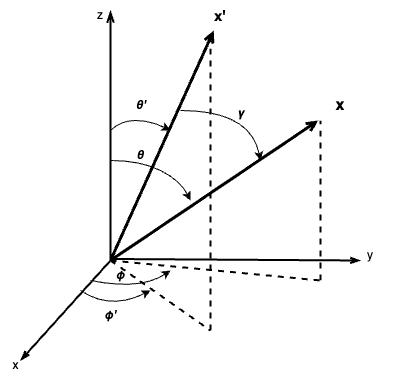
\includegraphics[width=0.4\textwidth]{figure/SphericalAdd.png}
    \caption{}
    \label{fig:fig1}
\end{figure}
为了计算这个系数,我们注意到,根据公式\ref{eq:3.60},它可以看作是函数 $\sqrt{4\pi/(2l + 1)} Y_l^m(\theta, \phi)$ 在以式\ref{eq:3.64} 中的参考轴(即带撇号的坐标轴)上的球谐函数 $Y_l^m(\gamma, \beta)$ 展开中 $m{\prime} = 0$ 的系数。由式\ref{eq:3.59} 可以发现,由于只有一个 $l$ 值存在,系数\ref{eq:3.66}表达为:
\begin{equation}\label{eq:3.67}
    A_m(\theta',\phi')=\frac{4\pi}{2l+1}\{Y_{lm}^{*}[\theta(\gamma,\beta),\phi(\gamma,\beta)]\}_{\gamma=0}
\end{equation}
当 $\gamma \to 0$ 时,角 $(\theta, \phi)$ 作为 $(\gamma, \beta)$ 的函数,将趋近于 $(\theta{\prime}, \phi{\prime})$。由此,附加定理 \ref{eq:3.62} 得证。有时该定理会使用 $\mathrm{P}l^m(\cos \theta)$ 的形式而不是 $Y_l^m$ 的形式来表示。此时,其形式为:
\begin{equation}\label{eq:3.68}
P_l(\cos \gamma) = P_l(\cos \theta) P_l(\cos \theta{\prime}) + 2 \sum{m=1}^l \frac{(l - m)!}{(l + m)!} \mathrm{P}_l^m(\cos \theta) \mathrm{P}_l^m(\cos \theta{\prime}) \cos[m(\phi - \phi{\prime})] \tag{3.68}
\end{equation}

若角度 $\gamma$ 趋于零,也可以推导出球协函数平方的“求和规则”:
\begin{equation}\label{eq:3.69}
    \sum_{m=-l}^l |Y_l^m(\theta, \phi)|^2 = \frac{2l + 1}{4\pi} \tag{3.69}    
\end{equation}

附加定理还可以用于将位于 $\mathbf{x}{\prime}$ 的单位电荷在 $\mathbf{x}$ 处产生的势的展开式\ref{eq:3.38}以最简洁的形式写出。

将式\ref{eq:3.62} 代入 $P_l(\cos \gamma)$,得到:
\begin{equation}\label{eq:3.70}
\frac{1}{|\mathbf{x} - \mathbf{x}{\prime}|} = 4\pi \sum_{l=0}^\infty \sum_{m=-l}^l \frac{1}{2l + 1} \left(\frac{r_<^l}{r_>^{l+1}}\right) Y_l^{m*}(\theta{\prime}, \phi{\prime}) Y_l^m(\theta, \phi) \tag{3.70}
\end{equation}

式 \ref{eq:3.70} 给出了坐标 $\mathbf{x}$ 和 $\mathbf{x}{\prime}$ 中因式分解的势形式。这对于涉及电荷密度积分的情况非常有用,其中一个变量是积分变量,另一个是观测点的坐标。然而,这样做的代价是用双重求和代替了单次求和。
\section{柱坐标系下的拉普拉斯方程;贝塞尔方程}
如图\ref{fig:cylin_coor}所示,在柱坐标系$(\rho,\phi,z)$下,拉普拉斯方程为如下的形式:
\begin{equation}\label{eq:3.71}
    \pderi{2}{\Phi}{\rho} + \frac{1}{\rho} \pderi{}{\Phi}{\rho} + \frac{1}{\rho^2} \pderi{2}{\Phi}{\phi} + \pderi{2}{\Phi}{z} = 0 
\end{equation}
\begin{figure}[h]
    \centering
    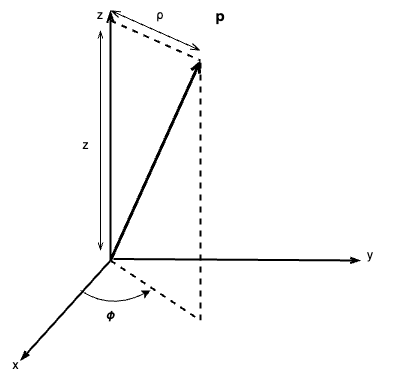
\includegraphics[width=0.4\textwidth]{figure/clyin_coor.png}
    \caption{}
    \label{fig:cylin_coor}
\end{figure}

变量分离由如下的变换给出:
\begin{equation}\label{eq:3.72}
    \Phi(\rho,\phi,z) = R(\rho) Q(\phi) Z(z)
\end{equation}
一般情况下,这将把上面的偏微分方程化为三个常微分方程:

    \begin{align}
        \deri{2}{Z}{z}-k^2Z &= 0 \\
        \deri{2}{Q}{\phi}+\nu^2Q &= 0 \\
        \deri{2}{R}{\rho}+\frac{1}{\rho}\deri{R}{\rho}+\left(k^2-\frac{\nu^2}{\rho^2}\right)R &= 0
    \end{align}

前两个常微分方程的解是基本的:
\begin{equation}\label{eq:3.74}
    \begin{aligned}
        Z(z)&=\ee^{\pm ikz} \\
        Q(\phi)&=\ee^{\pm i\nu\phi}
    \end{aligned}
\end{equation}
为了使势函数在整个方位角范围内是单值的,$\nu$ 必须是一个整数。但如果在 $z$ 方向没有任何边界条件的限制,参数 $k$ 是任意的。目前,我们假设 k 是实数且为正值。

径向的方程可以在变换$x=k\rho$下变为标准形式:
\begin{equation}\label{eq:3.75}
    \deri{2}{R}{x}+\frac{1}{x}\deri{R}{x}+\left(1-\frac{\nu^2}{x^2}\right)R=0
\end{equation}
这是贝塞尔方程的标准形式,该方程的解被称为$\nu$阶的贝塞尔函数。
假设解的形式为幂级数展开的形式:
\begin{equation}\label{eq:3.76}
    R(x)=x^\alpha\sum_{j=0}^{\infty}a_jx^J
\end{equation}
可以发现:
\begin{equation}\label{eq:3.77}
    \alpha = \pm \nu
\end{equation}
且对所有$j=1,2,3,\cdots$有:
\begin{equation}\label{eq:3.78}
    a_{2j}=-\frac{1}{4j(j+\alpha)}a_{2j-2}
\end{equation}
所有奇次项的系数都为零。这样,我们就可以通过递推法给出所有的系数:
\begin{equation}
    a_{2j}=\frac{(-1)^j\Gamma(\alpha+1)}{2^{2j}j!\Gamma(j+\alpha+1)}a_0
\end{equation}
传统上,我们取常数$a_0 = [2^\alpha \Gamma(\alpha+1)]^{-1}$,这样两个解就可以写成:

\begin{align}
    J_\nu (x) &= (\frac{x}{2})^\nu \sum_{j=0}^{\infty}\frac{(-1)^j}{j!\Gamma(j+\nu+1)}(\frac{x}{2})^{2j} \label{eq:3.82}\\
    J_{-\nu}(x) &= (\frac{x}{2})^{-\nu}\sum_{j=0}^{\infty}\frac{(-1)^j}{j!\Gamma(j-\nu+1)}(\frac{x}{2})^{2j}√\label{eq:3.83}
\end{align}

这两个解被称为$\pm\nu$阶的第一类贝塞尔函数。这个函数级数在任意的$x$都是收敛的。当$\nu$非整数时,这两个解$J_{\pm\nu}(x)$构成一组与二阶贝塞尔函数线性无关的解。然而,当$\nu$为整数时,非常显然这些解是线性相关的。
事实上,对于$\nu=m$($m$为整数)从级数的表达式可以看出:
\begin{equation}\label{eq:3.84}
    J_{-m}(x) = (-1)^m J_m(x)
\end{equation}
因此,当$\nu$为整数时,需要寻找另一个线性无关的解。即使$\nu$不是整数,通常也会用$J_\nu(x)$ 和 $N_\nu(x)$ 来替换 $J_{\pm\nu}(x)$,其中 $N_\nu(x)$ 是纽曼函数(或第二类贝塞尔函数):
\begin{equation}\label{eq:3.85}
    N_\nu(x) = \frac{J_\nu(x)\cos \nu\pi - J_{-\nu}(x)}{\sin \nu\pi}
\end{equation}
对于非整数的$\nu$,$N_\nu(x)$ 显然与 $J_\nu(x)$ 线性无关。在极限$\nu \to integer$时,可以证明 $N_\nu(x)$ 仍然与 $J_\nu(x)$ 线性无关。正如预期的那样,它与$\log{x}$有关。其级数表示在参考书中给出。

第三类贝塞尔函数,也成为汉克尔函数,是第一类贝塞尔函数$J_\nu(x)$和第二类贝塞尔函数$N_\nu(x)$的线性组合:
\begin{equation}\label{eq:3.86}
    \begin{cases}
        H_\nu^{(1)}(x) &= J_\nu(x) + iN_\nu(x) \\
        H_\nu^{(2)}(x) &= J_\nu(x) - iN_\nu(x)
    \end{cases}
\end{equation}
和 $J_\nu(x)$ 和 $N_\nu(x)$ 一样,汉克尔函数构成了贝塞尔方程的一组基本解。

函数 $J_\nu$、$N_\nu$、$H_\nu$,均满足递推公式:
\begin{align}\label{eq:3.88}
    \Omega_{\nu-1}(x) + \Omega_{\nu+1}(x) &= \frac{2\nu}{x} \Omega_{\nu}(x) \\
    \Omega_{\nu-1}(x) - \Omega_{\nu+1}(x) &= 2 \frac{d\Omega_{\nu}(x)}{dx}
\end{align}
其中 $\Omega_\nu(x)$ 是任意一个阶数为$\nu$的柱函数。这可以直接从级数表示\ref{eq:3.82}中验证。

为了方便参考,这里给出了各种贝塞尔函数在其参数取小量和较大值时的极限形式。为简便起见,我们仅展示领头阶项:
\begin{equation}
    \begin{aligned}
    x \ll 1 \quad J_\nu(x) &\to \frac{1}{\Gamma(\nu + 1)} \left( \frac{x}{2} \right)^\nu \\
    N_\nu(x) &\to
\begin{cases}
\frac{2}{\pi} \left[ \ln \left( \frac{x}{2} \right) + 0.5772 \cdots \right], & \nu = 0, \\
-\frac{\Gamma(\nu)}{\pi} \left( \frac{2}{x} \right)^\nu, & \nu \neq 0.
\end{cases}
\end{aligned}
\end{equation}
当$\nu$为非负实数。
\begin{equation}\label{eq:3.91}
    \begin{aligned}
    x \gg 1,\nu \quad J_\nu(x) &\to \sqrt{\frac{2}{\pi x}} \cos \left( x - \frac{\nu\pi}{2} - \frac{\pi}{4} \right)\\
    N_\nu(x) &\to \sqrt{\frac{2}{\pi x}} \cos \left( x - \frac{\nu\pi}{2} - \frac{\pi}{4} \right)
    \end{aligned}
\end{equation}
从$x$小量形式到$x$为较大量的渐近形式的过渡发生在$x \sim  \nu$的区域。

从渐近形式\ref{eq:3.91}可以清楚地看出,每个贝塞尔函数都有无限多个根。我们将主要关注$ J_\nu(x) $的根:
\begin{equation}\label{eq:3.92}
    J_\nu(x_{\nu,n}) = 0 \quad n = 1,2,3,\cdots
\end{equation}
$x_{\nu,n}$是$J_\nu(x)$的第 n 个根。对于前几个$\nu$取整数时,这里分别给出他们前几个根:
\[
\begin{aligned}
\nu = 0, \quad & x_{0n} = 2.405, \, 5.520, \, 8.654, \, \dots \\
\nu = 1, \quad & x_{1n} = 3.832, \, 7.016, \, 10.173, \, \dots \\
\nu = 2, \quad & x_{2n} = 5.136, \, 8.417, \, 11.620, \, \dots
\end{aligned}
\]
对于更高阶的根,它们的近似形式为:
\[
    x_{\nu,n} \approx \left( n + \frac{\nu}{2} - \frac{1}{4} \right) \pi
\]
该近似式提供了足够的精度(至少三位数字)。根的表格见于Jahnke,Emde and Losch(p.194)以及Abramowitz and Stegun(p.409)。

找到拉普拉斯方程径向部分的解并用贝塞尔函数表示后,我们可以进一步探讨贝塞尔函数在何种意义上构成一个正交且完备的函数集。
在这里,我们仅考虑第一类贝塞尔函数,并证明当$\nu > 0$固定且$n = 1,2,3,\dots$时,函数$\sqrt{\rho}J_\nu(x_{\nu,n}\rho/a)$在区间$0<\rho<a$上构成一个正交集。先从$J_\nu(x_{\nu,n}\frac{\rho}{a})$满足的微分方程开始:
\begin{equation}
    \frac{1}{\rho} \frac{d}{d\rho} \left[ \rho \frac{dJ_\nu\left( x_{\nu n} \frac{\rho}{a} \right)}{d\rho} \right] + \left( \frac{x_{\nu n}^2}{a^2} - \frac{\nu^2}{\rho^2} \right) J_\nu\left( x_{\nu n} \frac{\rho}{a} \right) = 0
\end{equation}
如果我们将该微分方程乘上$\rho J_\nu(x_{\nu n'}\rho/a)$并从 0 积分到 $a$,我们可以得到:
\[
\int_0^a J_\nu\left(x_{\nu n'} \frac{\rho}{a}\right) \frac{d}{d\rho} 
\left[
\frac{dJ_\nu\left(x_{\nu n} \frac{\rho}{a}\right)}{\rho \, d\rho}
\right] d\rho
+ \int_0^a \left( \frac{x_{\nu n}^2}{a^2} - \frac{\nu^2}{\rho^2} \right) \rho J_\nu\left(x_{\nu n'} \frac{\rho}{a}\right) J_\nu\left(x_{\nu n} \frac{\rho}{a}\right) d\rho = 0
\]
使用分部积分法,并应用$(\rho J_\nu J'_\nu)$在$\rho = 0$和$a$处为0,得到以下的结果:
\[
- \int_0^a \rho \frac{dJ_\nu\left(x_{\nu n'} \frac{\rho}{a}\right)}{d\rho}
\frac{dJ_\nu\left(x_{\nu n} \frac{\rho}{a}\right)}{d\rho} \, d\rho
+ \int_0^a \left( \frac{x_{\nu n}^2}{a^2} - \frac{\nu^2}{\rho^2} \right)
\rho J_\nu\left(x_{\nu n'} \frac{\rho}{a}\right) J_\nu\left(x_{\nu n} \frac{\rho}{a}\right) \, d\rho = 0
\]
交换$n$和$n'$的标记,并与上式相加减,我们就得到正交性条件:
\begin{equation}\label{eq:3.94}
    (x_{\nu n}^2 - x_{\nu n'}^2)\int_0^a \rho J_\nu(x_{\nu n'},\frac{\rho}{a})J_\nu(x_{\nu n},\frac{\rho}{a})\ d\rho = 0
\end{equation}
巧妙地使用微分方程以及递归公式\ref{eq:3.88} 可以得到归一化积分:
\begin{equation}\label{eq:3.95}
    \int_0^a \rho J_\nu(x_{\nu n'},\frac{\rho}{a})J_\nu(x_{\nu n},\frac{\rho}{a})\ d\rho = \frac{a^2}{2} \left[ J_{\nu+1}(x_{\nu n}) \right]^2 \delta_{nn'}
\end{equation}
假设贝塞尔函数的集合是完备的,我们可以在区间$0<\rho<a$上将任意关于$\rho$函数展开为傅里叶-贝塞尔级数:
\begin{equation}\label{eq:3.96}
    f(\rho) = \sum_{n=1}^{\infty} A_{\nu n}  J_\nu(x_{\nu n}\frac{\rho}{a})
\end{equation}
其中系数$A_{\nu n}$由下式给出:
\begin{equation}\label{eq:3.97}
    A_{\nu n} = \frac{2}{a^2 J_{\nu+1}^2(x_{\nu n})} \int_0^a \rho f(\rho) J_\nu(x_{\nu n}\frac{\rho}{a})\ d\rho
\end{equation}
我们对\ref{eq:3.96}的推导涉及了限制条件$\nu > 0$。实际上,可以证明它对所有$\nu \geq  -1$都成立。

展开式\ref{eq:3.96}和\ref{eq:3.97}是常规的傅里叶-贝塞尔级数,特别适用于在$\rho =a$时为 0 的函数(例如,圆柱体上的齐次狄利克雷边界条件;见下节)。
但需要注意的是,也可以用函数系$\sqrt{\rho}J_\nu y_{\nu n}\rho /a$进行展开,其中 $y_{\nu n}$ 是方程 $[dJ_\nu(x)]/dx = 0$ 的第 n 个根。原因在于,在证明这些函数的正交性时,只需满足量 $[\rho J_\nu(k\rho)(d/d\rho)J_\nu(k\rho)-\rho J_\nu(k'\rho)(d/d\rho)J_\nu(k\rho)]$ 在端点 $\rho = 0$ 和 $\rho = a$ 时为 0。
这个要求可以通过$\lambda = x_{\nu n}/a$或 $\lambda = y_{\nu n}/a$ 来满足,其中 $J_\nu(x_{\nu n}) = 0;J'_\nu (y_{\nu n})=0$。更一般地,通过在端点处满足 $\rho(d/d\rho)J_\nu(k\rho) + \lambda J_\nu(k\rho) = 0$,其中 $\lambda$ 是一个与 $k$ 无关的常数。以 $\sqrt{\rho}J_\nu (y_{\nu n}\rho/a)$ 为基础的展开对于在 $\rho = a$ 时斜率为零的函数尤其有用。(见问题 3.11。)

傅里叶-贝塞尔级数只是涉及贝塞尔函数的一种展开形式。其他的形式包括:

纽曼级数:$\sum_{n=0}^\infty a_n J_{\nu + n}(z)$

Kepteyn级数:$\sum_{n=0}^\infty a_n J_{\nu +n}((\nu + n)z)$

Schl\"{o}milch级数:$\sum_{n=0}^\infty a_n J_{\nu}(nx)$

读者可以参考Watson(第十六至十九章)以获取关于这些级数性质的详细讨论。Kapteyn 级数出现在行星开普勒运动和快速移动电荷辐射的讨论中(见问题 14.14 和 14.15)。

在结束贝塞尔函数性质的讨论前,我们注意到,如果在拉普拉斯方程的分离变量过程中,将\ref{eq:3.74}中的分离常数 $k^2$ 取为 $-k^2$,那么 $Z(z)$ 将会是 $\sin(kz)$ 或 $\cos (kz)$,而 $R(\rho)$ 的方程将会是:
\begin{equation}
    \deri{2}{R}{\rho}+\frac{1}{\rho}\deri{}{R}{\rho}-\left(k^2+\frac{\nu^2}{\rho^2}\right)R=0
\end{equation}\label{eq:3.98}
在代换$k\rho = x$下:
\begin{equation}\label{eq:3.99}
    \deri{2}{R}{x}+\frac{1}{x}\deri{}{R}{x}-\left(1+\frac{\nu^2}{x^2}\right)R=0
\end{equation}
这个方程的解称为修正贝塞尔函数。显然,它们只是纯虚数参数的贝塞尔函数。通常选择该方程的两个线性独立解:$I_\nu(x)$ 和 $K_\nu(x)$ 表示。它们的定义为:
\begin{equation}\label{eq:3.100}
    \begin{aligned}
    I_\nu(x) &= i^{-\nu} J_\nu(ix) \\
    K_\nu(x) &= \frac{\pi}{2} i^{\nu+1} H_\nu^{(1)}(ix)
    \end{aligned}
\end{equation}
它们对于实数$x$和$\nu$是实函数。假设 $\nu \geq 0$,它们在$x$ 为小量和极大的极限形式为:
\begin{align}
    x &\ll 1 \\
    I_\nu(x) &\to \frac{1}{\Gamma(\nu + 1)}\left(\frac{x}{2}\right)^\nu \left[-\ln\left(\frac{x}{2}\right) + 0.5772 \dots\right] \\
    K_\nu(x) &\to \left\{\begin{array}{ll}
    \frac{1}{\Gamma(\nu)}\left(\frac{2}{x}\right)^\nu & \text{if } \nu = 0 \\
    \frac{1}{\Gamma(\nu)}\left(\frac{2}{x}\right)^\nu & \text{if } \nu \neq 0
    \end{array}\right. \\
    x &\gg 1, \nu \\
    I_\nu(x) &\to \frac{1}{\sqrt{2\pi x}}\mathrm{e}^{x}\left[1 + \mathcal{O}\left(\frac{1}{x}\right)\right] \\
    K_\nu(x) &\to \sqrt{\frac{\pi}{2x}}\mathrm{e}^{-x}\left[1 + \mathcal{O}\left(\frac{1}{x}\right)\right]
\end{align}
\end{document}

